—————————————————————————————————————————————————————————————————————————————————————\\
\begin{center}
	\textbf{\LARGE{Lilypond}}
\end{center}
Endroit pour les fichiers de la drum :\\
/home/martin/lilypond/usr/share/lilypond/current/ly/drumpitch-init.ly\\\\
—————————————————————————————————————————————————————————————————————————————————————\\\\
\subsection{Écriture de partitions}
Les partitions pour la transcription manuelle seront écrites avec LilyPond.\\\\
Voici un exemple de code :
\begin{verbatimtab}
	\version "2.22.1"
	\language français
	{
		do' re' mi' fa' sol' la' si' do'' re'' mi'' fa'' sol'' la'' si'' do'''
	}
	\relative {
		do' re mi fa sol la si do re mi fa sol la si do
	}
	\relative {
		do'4. do4. do4
		mi2 re
		do16 do do do do do8 do16 do do do do do do8 do16
		mi8 mi mi mi re re re re
	}
\end{verbatimtab}
Avec la commande :\begin{verbatim}$ lilypond fichier.ly\end{verbatim}:
On obtient le pdf suivant :\\
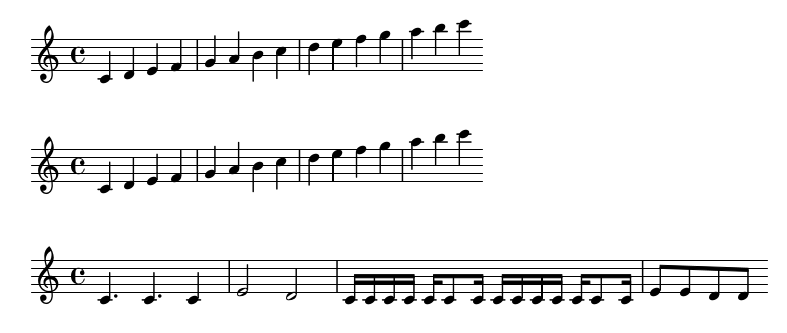
\includegraphics[height=50mm, width=110mm]{images/lilypond_0.png}\\\\
\textbf{Bases :}\\
\url{http://lilypond.org/doc/v2.22/Documentation/learning/simple-notation}\\

\textbf{Percussions et batterie :}\\
\url{http://lilypond.org/doc/v2.22/Documentation/notation/common-notation-for-percussion}

La définition des symboles a été faite avec lilypond avec le script suivant :
\begin{verbatimtab}
	$ cat description_notation_0.ly 
	
	\version "2.22.1"
	\language français
	
	{
		% Toutes les hauteurs sont en ut
		\clef percussion
		
		% Ne pas appeler la fonction qui dessine les symboles
		\override Staff.TimeSignature.stencil = ##f 
		
		% Changer la tête de note
		\override NoteHead.style = #'cross
		
		% Hauteur de la note + commentaire
		do''-"ride"
	}
	
	{
		\clef percussion
		\override Staff.TimeSignature.stencil = ##f
		\override NoteHead.style = #'cross
		la'-"charley main"
	}
	
	{
		\clef percussion
		\override Staff.TimeSignature.stencil = ##f
		fa'-"tom alto"
	}
	
	{
		\clef percussion
		\override Staff.TimeSignature.stencil = ##f
		do'-"caisse claire"
	}
	
	{
		\clef percussion
		\override Staff.TimeSignature.stencil = ##f
		sol-"tom basse"
	}
	
	{
		\clef percussion
		\override Staff.TimeSignature.stencil = ##f
		mi-"grosse caisse"
	}
	
	{
		\clef percussion
		\override Staff.TimeSignature.stencil = ##f
		\override NoteHead.style = #'cross
		do-"charley pied"
	}
\end{verbatimtab}